\documentclass[11pt]{rapport-tp-qlm}
% Pour les documents écrits en général, entre 10pt et 12pt
% 11pt OBLIGATOIRE POUR LE RAPPORT de l'UE Devenir Étudiant.e

% Bonne lecture des lettres accentuées :
\usepackage[utf8]{inputenc}
% si ça ne marche pas sur des systèmes un peu anciens, à la place
% de [utf8] on peut essayer [cp1252] sur Windows, ou [latin1] sur
% Mac ou Linux / Ubuntu / Fedora

% Choix d'une police de caractères :
\usepackage{lmodern}
% Dizaines d'autres possibilités, par exemple iwona, charter... 
% Voir par exemple  http://www.tug.dk/FontCatalogue/mathfonts.html
\usepackage[T1]{fontenc} % Nécessaire avec certaines police
\usepackage[section]{placeins}
% Les paquets suivants permettent d'inclure des liens internets,
% des images, des pages pdf :
\usepackage{hyperref}
\usepackage{graphicx}
\usepackage{pdfpages}
\usepackage{listings}
\usepackage{float}
\usepackage{graphicx}
\graphicspath{ {./assets/} }
%%%%%%%  FIN DE L'EN-TÊTE - DÉBUT DU CONTENU %%%%%%
\begin{document}


\title{Rapport TP 3 - IFT3913}

\author{
	\\Loïc Daudé Mondet
	\\20243814 -- Programmes d'échanges - 1er c.(Échange)
	\\
	\\Alaa edlin Yacoub
}

\date{18/11/2022}

\maketitle

\chapter{Boîtes à moustache et distribution des données}
    \section{NOCom}
    \begin{figure}[h]
    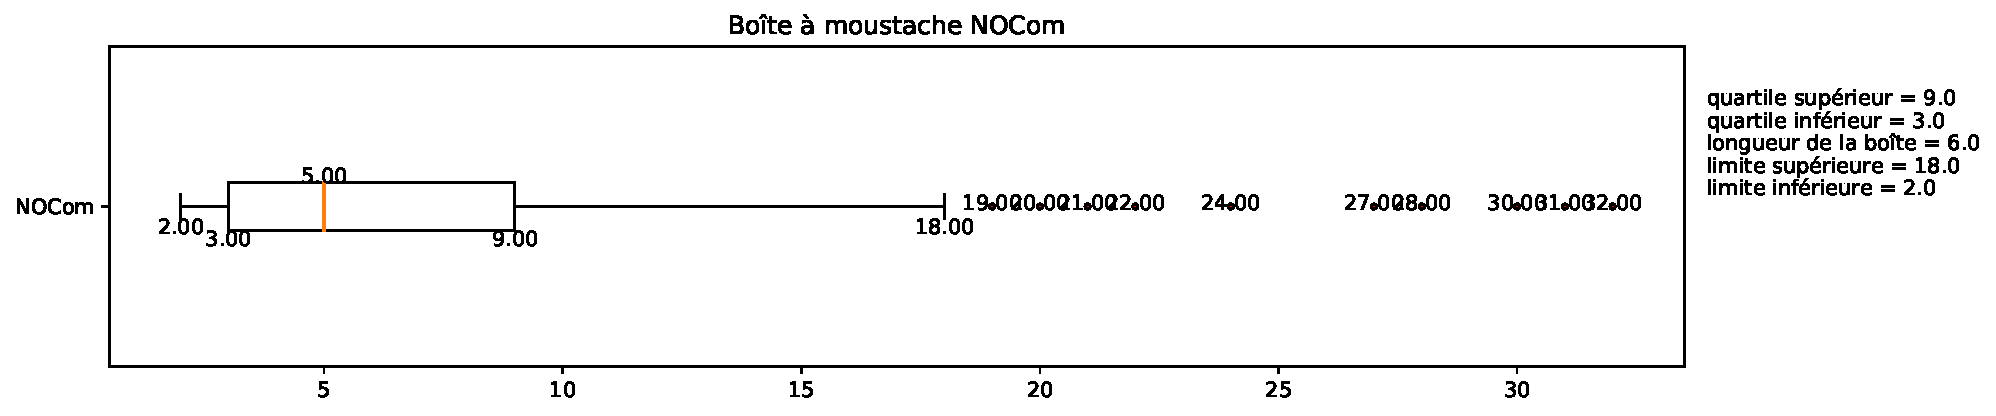
\includegraphics[scale=0.5]{assets/moustache_NOCom}
    \centering
    \end{figure}
    La boîte n'est pas symétrique ce qui signifie que les variables ne sont pas normalement distribuées, conclusion renforcée par le grand nombre de valeurs extrêmes.
    \section{NCLOC}
    \begin{figure}[h]
    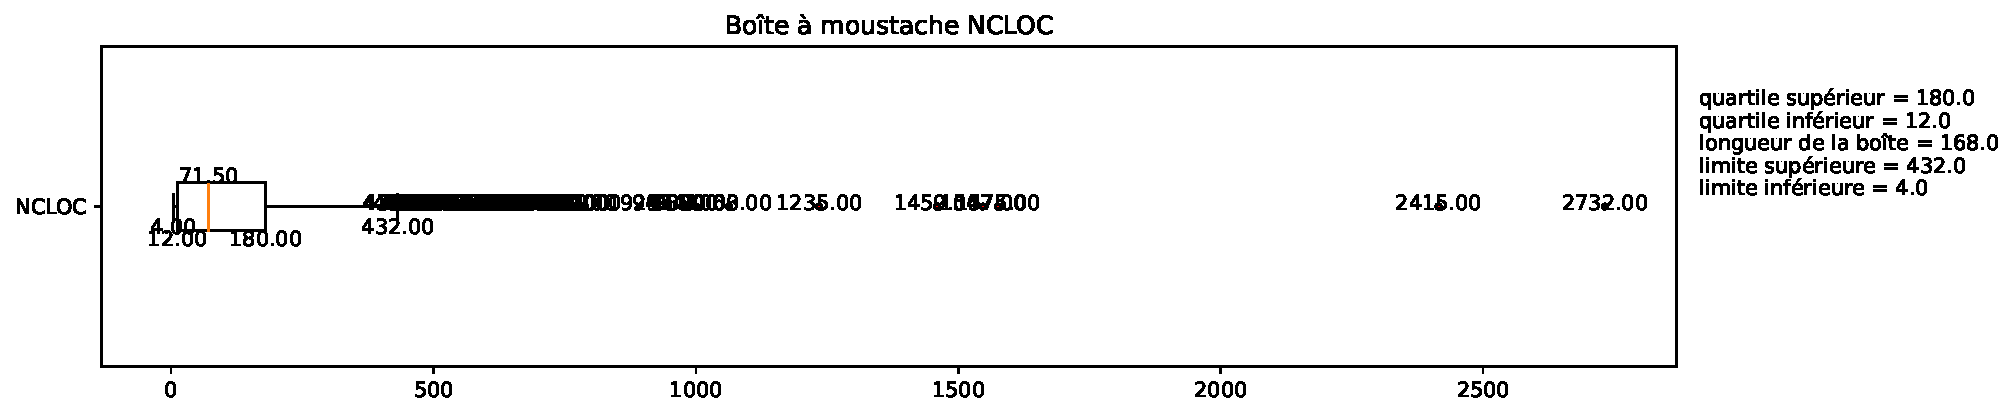
\includegraphics[scale=0.5]{assets/moustache_NCLOC}
    \centering
    \end{figure}
       Ici aussi, la boîte n'est pas symétrique et les variables ne sont donc encore une fois pas normalement distribuées, de plus on observe un nombre encore plus élevé de valeurs extrêmes. 
     \newpage
    \section{DCP}
    \begin{figure}[h]
    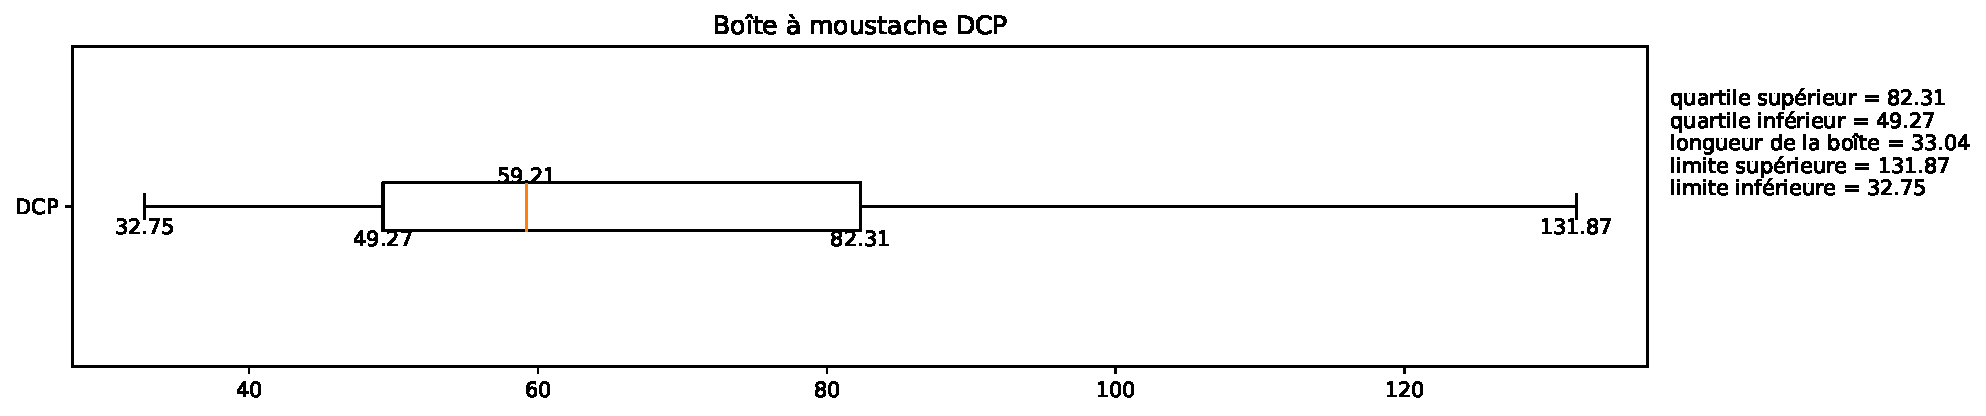
\includegraphics[scale=0.5]{assets/moustache_DCP}
    \centering
    \end{figure}
  Pour DCP, la boite bien que toujours asymétrique, les longueurs des moustaches sont sensiblement plus proches que dans les cas précédents et le placement de la médiane dans la boite est également plus centré, on note également l'absence de valeurs extrêmes, cela traduit donc une distribution des variables plus proche d'une distribution suivant la loi normale.
  
\chapter{Correlations}
    \section{NCLOC en fonction de NOCom}
    \begin{figure}[h]
    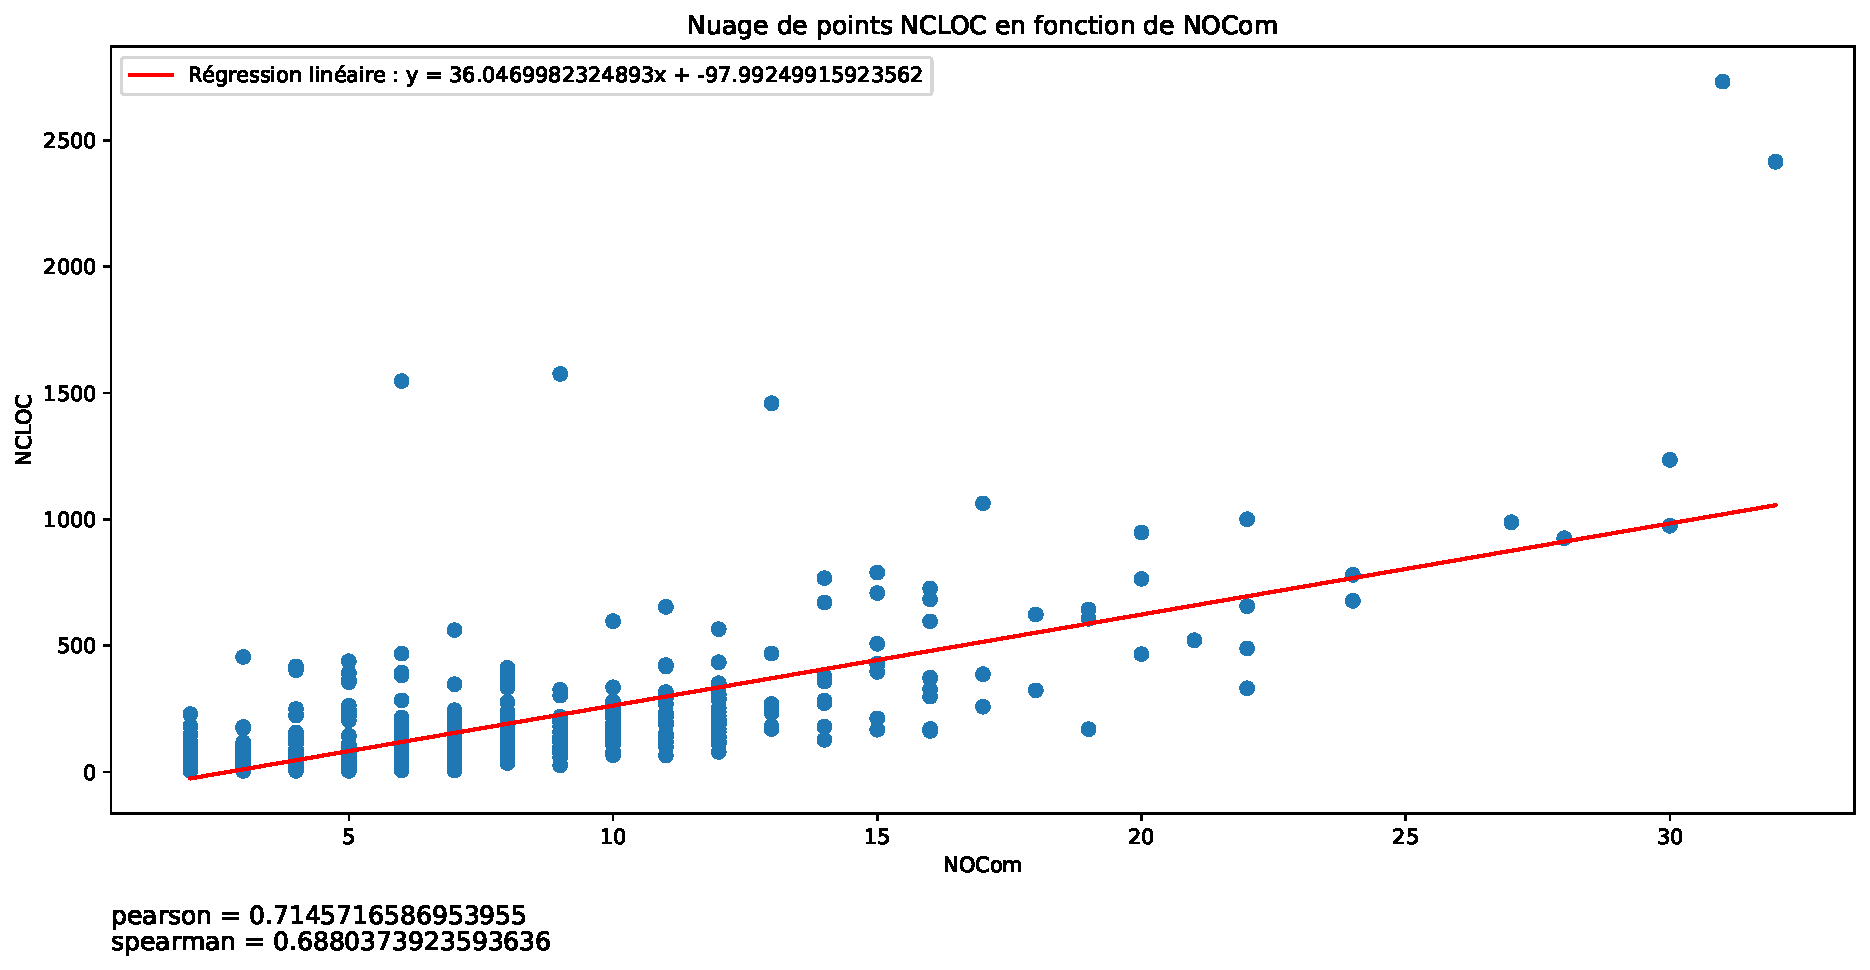
\includegraphics[scale=0.5]{assets/relation_NCLOC_NOCom}
    \centering
    \end{figure}
    On remarque que la plupart des points du graphique représentant NCLOC en fonction de NOCom semblent se répartir autour et en suivant une droite. Comme les variables ne sont pas normalement distribuées (cf la partie précédente), on utilise le coefficient de corrélation de Spearman et on trouve 0.688 ce qui témoigne d'une certaine relation relativement linéaire entre ces deux métriques puisque cette valeur est plus proche de 1 que de 0. On trouve alors en effectuant la régression linéaire l'équation suivante y = 36,05x - 97,99 décrivant cette relation.
     \newpage
    \section{DCP en fonction de NOCom}
 
    \begin{figure}[h]
    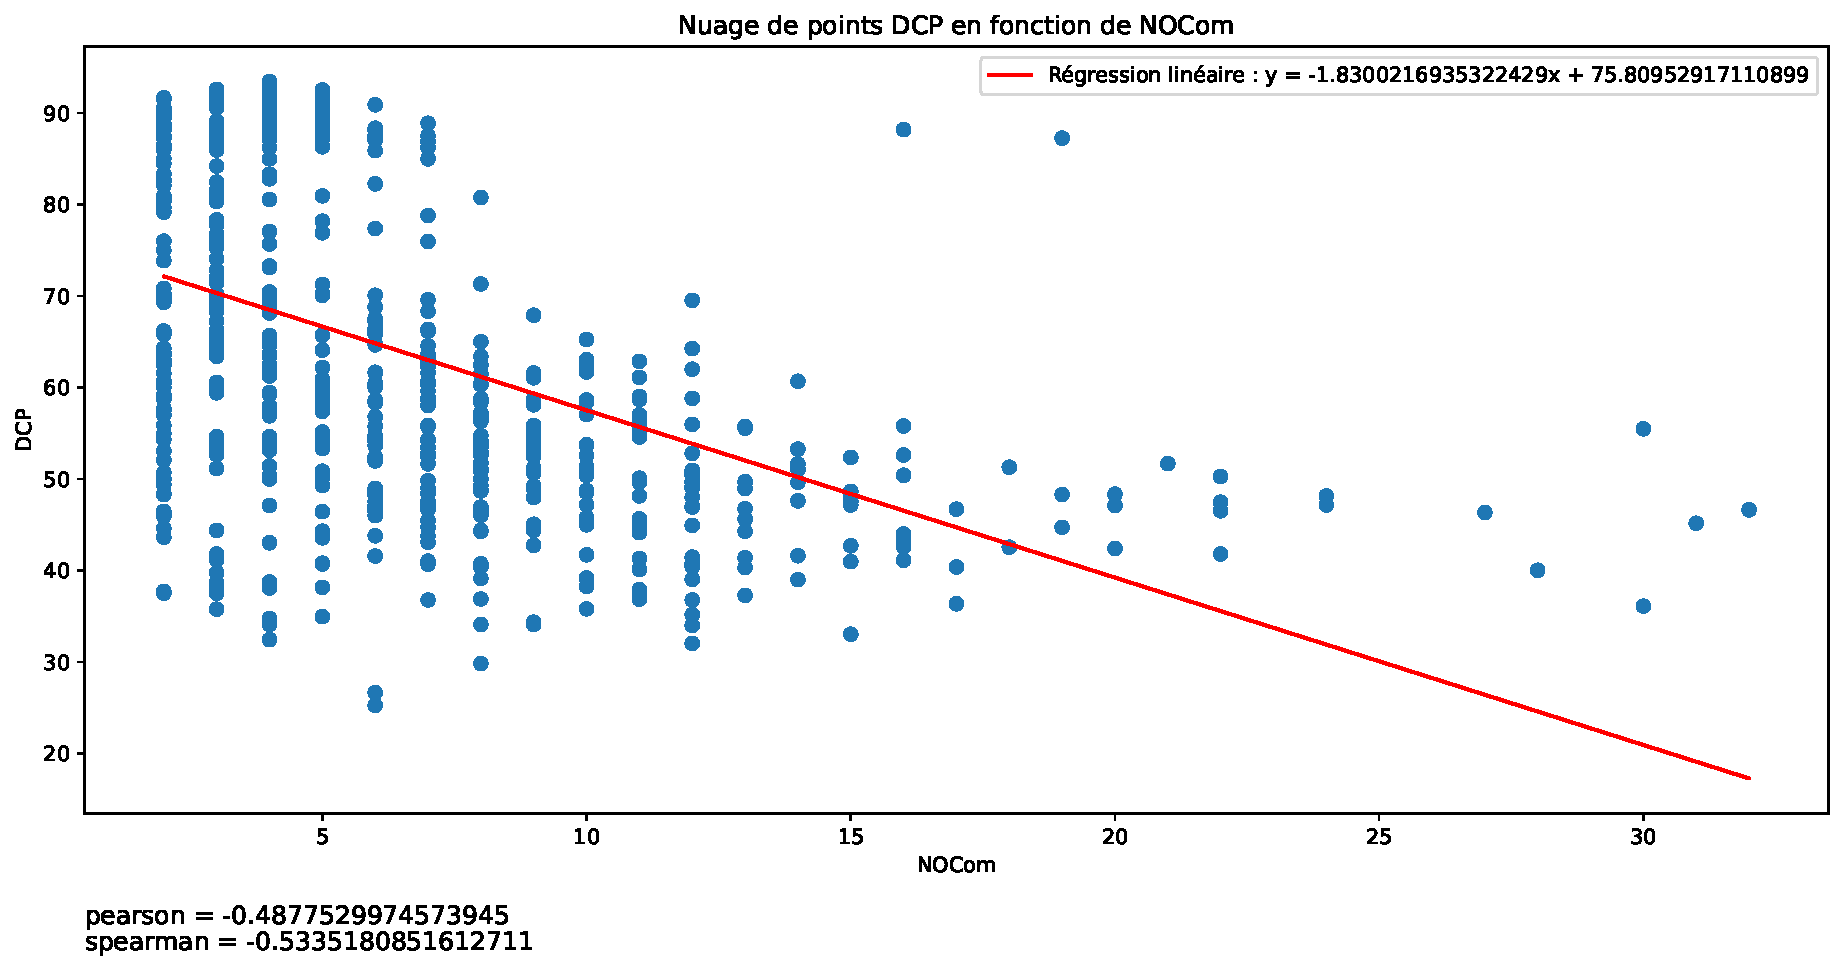
\includegraphics[scale=0.5]{assets/relation_DCP_NOCom}
    \centering
    \end{figure}

Ici, les points ne semblent pas vraiment suivre une même droite, cette observation est confirmée par la valeur de -0,53 du coefficient de Spearman qui bien que légèrement plus proche de -1 que de 0 ne constitue pas une valeur témoignant d'une relation très proche de la linéarité entre les deux métriques. Si on essaye toutefois d'obtenir une régression linéaire entre ces deux variables, on trouve l'équation y = -1,830x + 75,80.
    
\chapter{Quasi expérience}
Hypothèse : << les classes qui ont été modifiées plus de 10 fois sont mieux commentées que celles qui ont été modifiées moins de 10 fois >>

\end{document}